\section{Summary}
COVID-19 has been one of the most severe pandemics in recent history developing a dynamic that is very hard to model let alone understand. With only limited data available, this calls for sophisticated methods to perform inference on the driving factors of the disease and assess the efficacy of non-pharmaceutical interventions. In their paper 'Bayesian inference of COVID-19 spreading rates in South Africa' R. Mbuvha and T. Mawala use a Markov-Chain Monte Carlo method to examine the impacts of governmental measures to reduce the spread of the virus. Their main finding are two change points in the course of the disease that constitute changes in the spreading rate corresponding to enactments of governmental restrictions. 
\newline \newline
The models that are used to perform inference on are given by compartmental methods. These are characterised by modelling the transitions between various stages of the disease. More specifically, R. Mbuvha and T. Mawala consider the Susceptible-Exposed-Infectious-Recovered  (SEIR) and the its simplification the Susceptible-Infectious-Recovered (SIR) models. The SEIR model can be respresented as a four-state Markov chain as illustrated in figure \ref{V1}.

\begin{figure}[h]
	\centering
	
\includegraphics[width = 0.7\textwidth]{V1}
	\caption{SEIR model \cite{Bayes}}
	\label{V1}
\end{figure}
\noindent It is governed by the following system of ODEs:
\begin{align}
	\frac{dS}{dt} & = - \frac{\lambda S I }{N} \\
	\frac{dE}{dt} & = \frac{\lambda SI }{N} - \sigma E \\
	\frac{dI}{dt} & = \sigma E - \mu I \\
	\frac{dR}{dt} & = \mu I
\end{align}
where $S,E,I,R$ are the respective populations belonging to the above classes and $N$ is the total population. Another key quantity in the S(E)IR model is the basis reproductive number that represents the mean number of additional infections caused by one infected individual:
\begin{equation}
R_0 = \frac{\lambda}{\mu}
\end{equation}
Furthermore, the model is extended by a delay in becoming infected ($I^\text{new}$) and being reported and the spreading rate $\lambda$ is assumed to be time-varying after according to some check-points that are affected by governmental interventions.
\newline \newline
To perform inference, appropriate priors and likelihood functions need to be specified. The likelihood function was chosen to be a Student-T distribution which resembles a Gaussian around the mean, but makes the MCMC more robust to outliers. The priors for the respective parameters are based on literature based expected values of parameters and are summarised in figure \ref{V2}.
\begin{figure}[h]
	\centering
	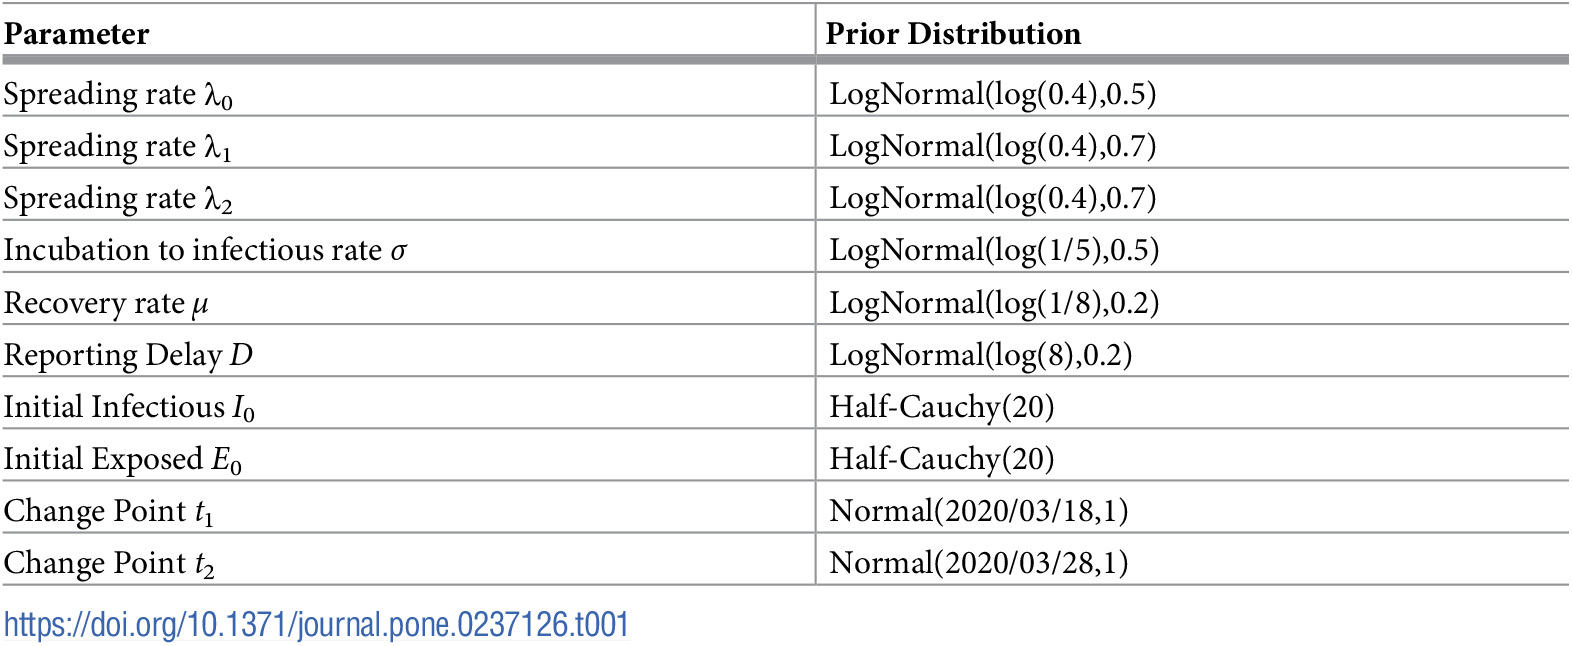
\includegraphics[width = 0.7\textwidth]{V2}
	\caption{Prior distributions \cite{Bayes}}
	\label{V2}
\end{figure}
A Markov-Chain Monte Carlos algorithm is used to sample from the posterior, since closed-form inference is infeasible. More specifically, the authors adopted the Hamiltonian Monte Carlo (HMC) method - a variation of the classical Metropolis-Hastings (MH) algorithm. In high dimensions, the chain produced by MH tends to get stuck and autocorrelation between the samples is high. HMC overcomes this problem by making use of the geometry of the target distribution to propose samples that lie in the typical set; thus increasing the acceptance probability and traversing the typical set more efficiently. 
Finally, HMC is supplemented by No-U-Turn Sampling (NUTS), which automates the tuning of the leapfrog setpsize for integration and the trajectory length. 
\newline \newline 
The results are obtained by drawing 5000 samples from the Markov-chain with 1000 burn-in steps. Figure \ref{V3} shows that the SIR model with two change points yields the lowest mean Leave-one out (LOO) cross entropy loss among the different models.
\begin{figure}[h]
	\centering
	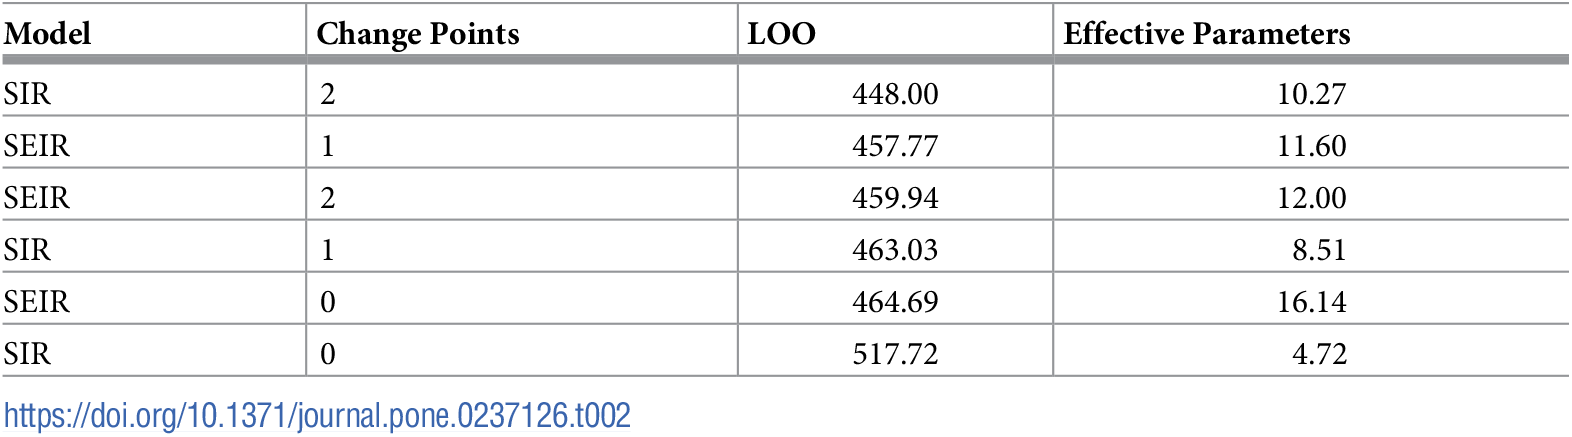
\includegraphics[width = 0.8\textwidth]{V3}
	\caption{Model comparisons \cite{Bayes}}
	\label{V3}
\end{figure}
To investigate the impact of governmental restrictions, the results of the posterior distribution produced by the 2 change point SIR model are summarised in figure \ref{V5}.

\begin{minipage}{0.4\textwidth}
	We see that the posterior estimates of the change points peak at the mean date of 18 March 2020, when the travel ban, school closures and social distancing recommendations were imposed. The date of the second change point peaks on 28 Match 2020, when mass screening and testing was announced. Furthermore, we infer a substantial drop in the spreading rate (80\% and 60\% from the initial value respectively) after the change dates. This corresponds to $R_0$ values of 3.278 (CI[2.715, 3.73]), 0.655 (CI[0.430, 0.960]) and 1.304 (CI[0.887, 1.7748]) at the respective change points. The rise in the $R_0$ value from the first to the second change point could be attributed to a widen-
\end{minipage}
\begin{minipage}[c]{0.6\textwidth}
	\centering
	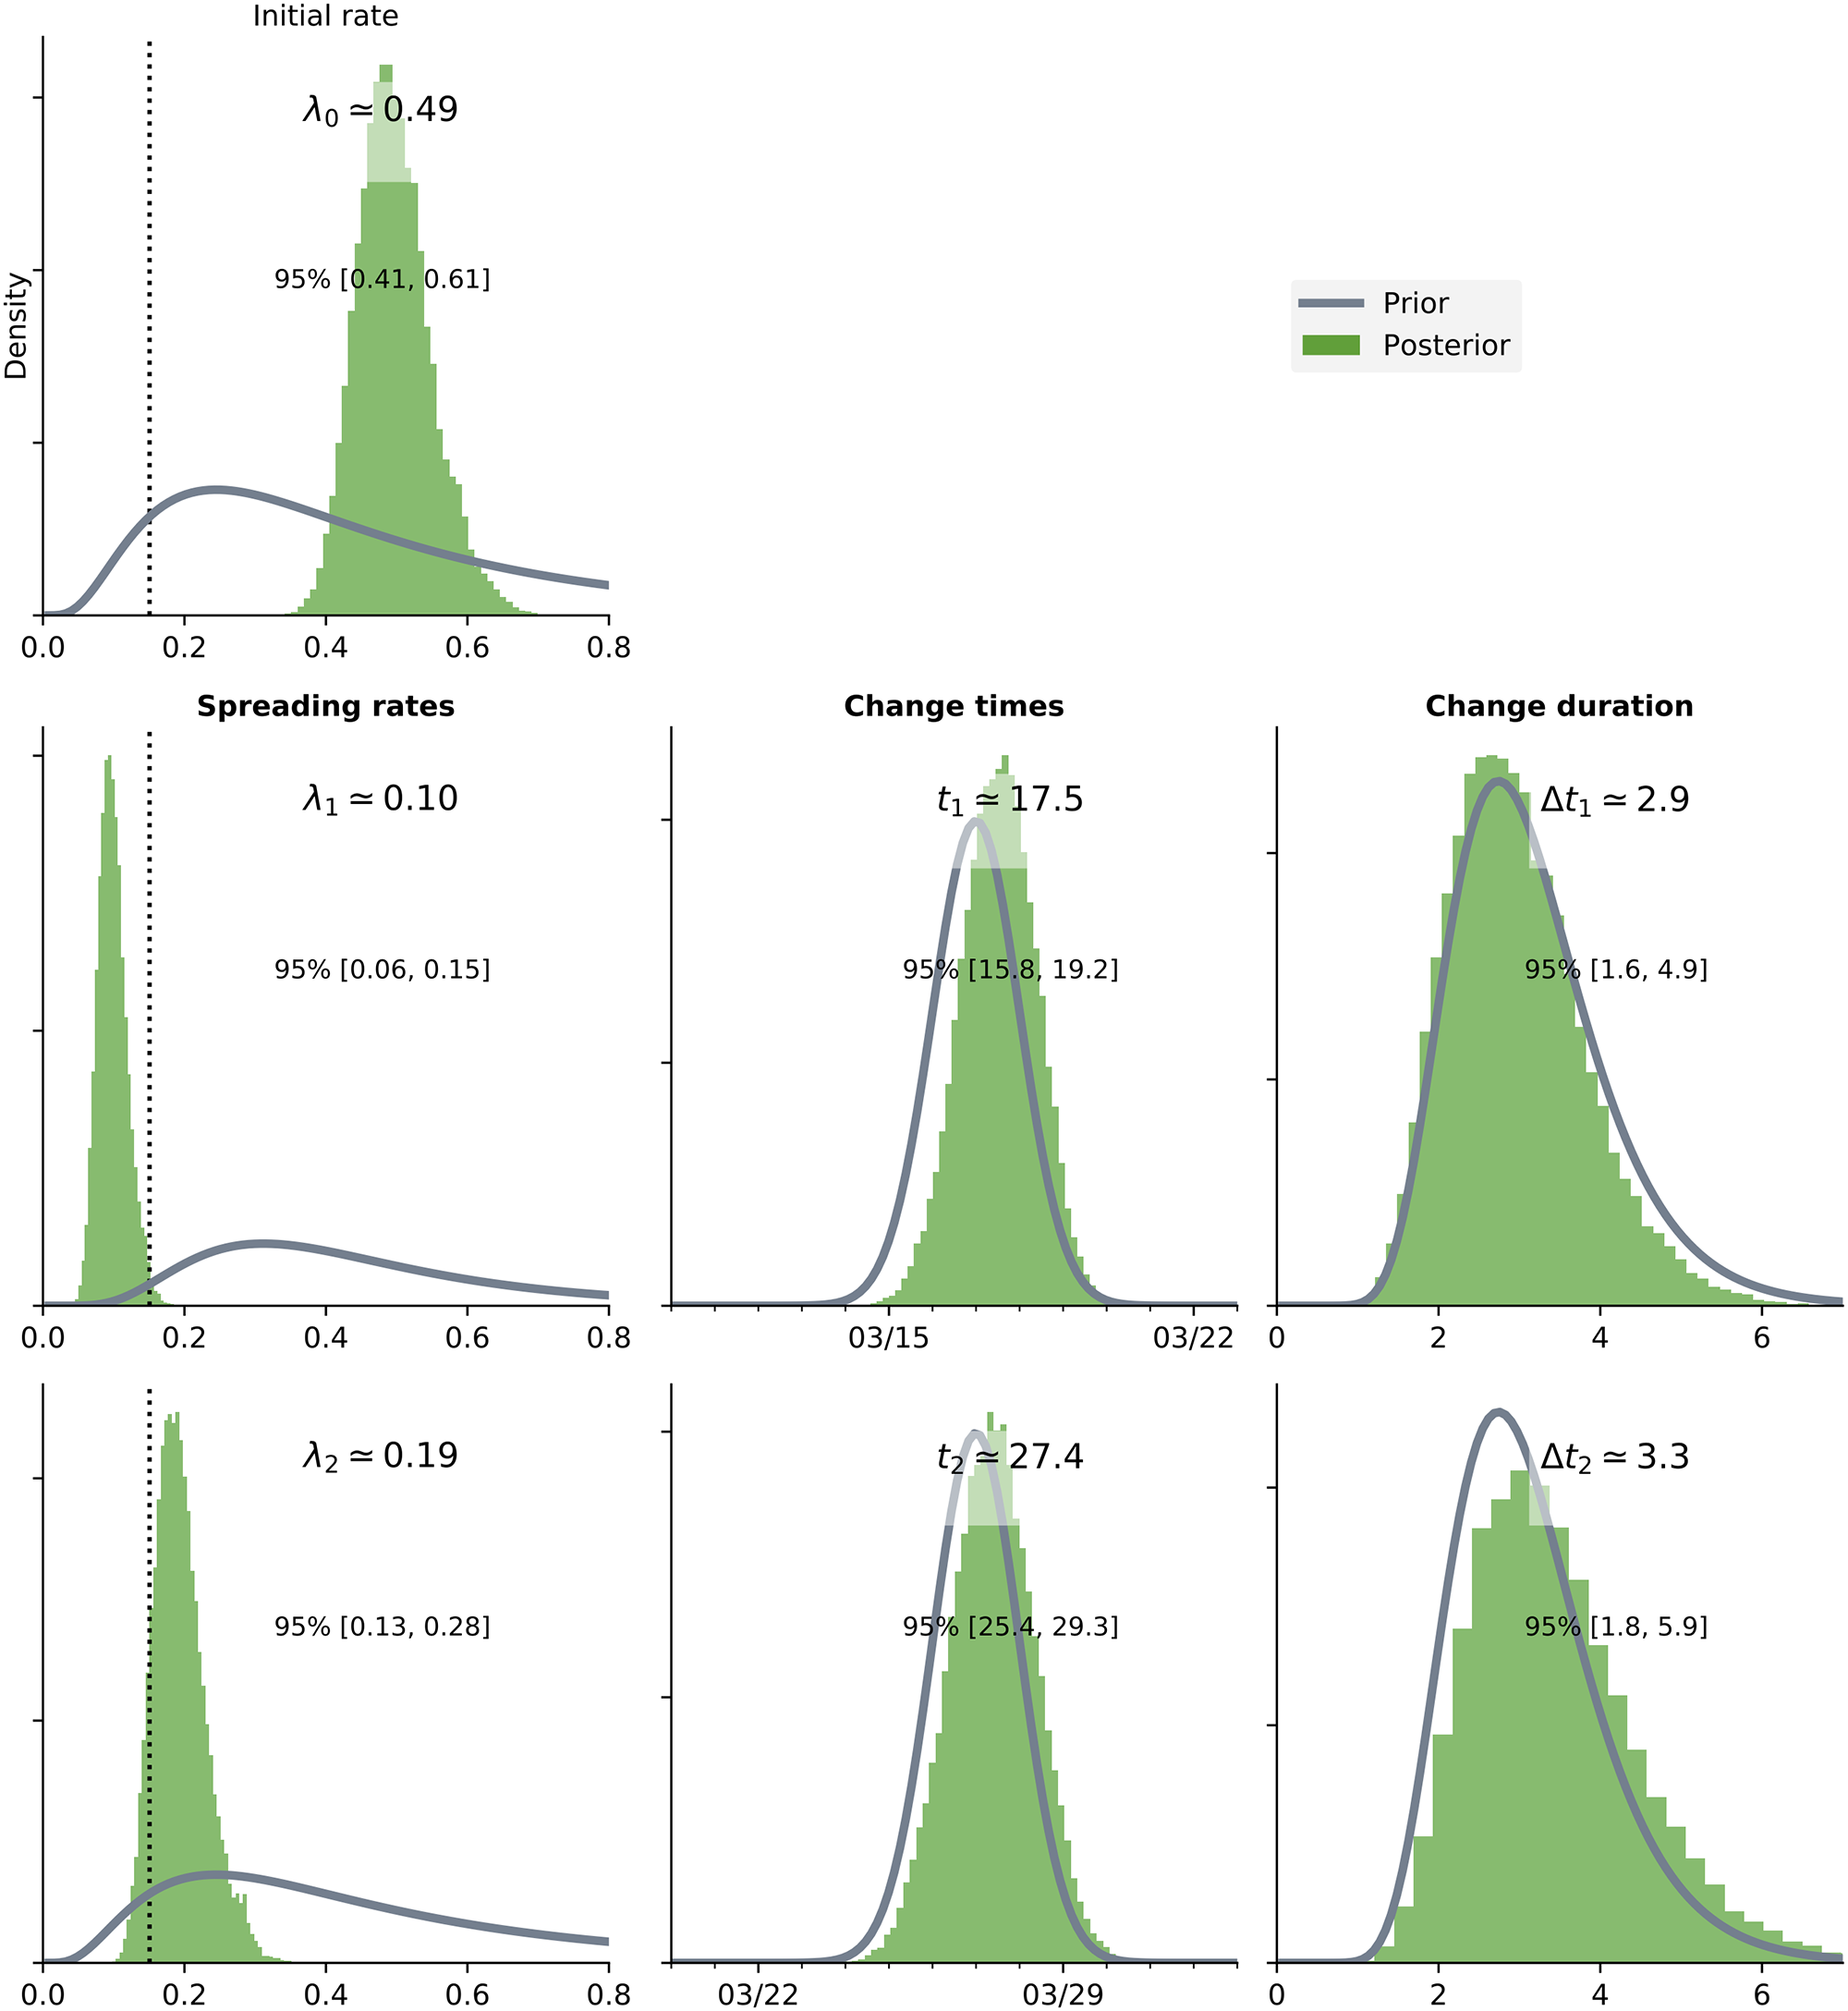
\includegraphics[width=0.9\textwidth]{V5}
	\captionof{figure}{Posterior distribution of parameters}
	\label{V5}		
\end{minipage}
\newline \newline
ing of the population eligible for testing. The mean reporting delay was found to be 6.848 (CI[5.178, 8.165]). A mean recovery rate $\mu \approx 0.151$ implies a mean infectious period of 6.62 days aligning with literature results. 
\newline \newline
To conclude, we note that the results imply an impact of governmental restrictions on the spreading rate. The estimated change dates correspond to the actual dates on which the government imposed further restrictions and a change in the $R_0$ value was found. I am personally very much in favor of Bayesian models as they provide a powerful tool to infer parameter values based on observations. However, it's always important to be aware of potential assumptions made in the prior distribution as the results can be quite sensitive to such assumptions. For example, I am wondering, what the exact form of the full prior is that the authors used. Additional improvements to the proposed method could be to take into account local, provincial developments providing a finer model.